\documentclass{osa-article}

%% Select the journal you're submitting to
%% oe, boe, ome, osac, osajournal
\journal{oe}
% Key:
% Express journals must have the correct journal selected:
% {oe} Optics Express
% {boe} Biomedical Optics Express
% {ome} Optical Material Express
% {optcon} Optics Continuum
% Other OSA journals may use:
% {osajournal} Applied Optics, Advances in Optics and Photonics, Journal of the Optical Society of America A/B, Optics Letters, Optica, Photonics Research

% Uncomment if submitting to Photonics Research.
% ONLY APPLICABLE FOR \journal{osajournal}
% \setprjcopyright

% Set the article type
%\articletype{Research Article}
% Note that article type is not required for Express journals (OE, BOE, OME and OSAC)
% \usepackage[hang,small,bf]{caption}
\usepackage[subrefformat=parens]{subcaption}
\captionsetup{compatibility=false}
\usepackage{todonotes}
\usepackage{lineno}
\usepackage{layout}
\usepackage{lipsum}
\usepackage{bm, amsmath, comment, color, soul, cite, siunitx, physics}
\sisetup{parse-numbers = false}
\linenumbers

\begin{document}

\title{Untitled}

\author{Yasutaka IMAI,\authormark{1, *}, Hideaki HARA,\authormark{1, *}}

\address{\authormark{1}Reserch Institute for Interdisciplinary Science, Okayama University, Okayama, Japan}

\email{\authormark{*}imai1117@okayama-u.ac.jp} %% email address is required

% \homepage{http:...} %% author's URL, if desired

%%%%%%%%%%%%%%%%%%% abstract %%%%%%%%%%%%%%%%
%% [use \begin{abstract*}...\end{abstract*} if exempt from copyright]
\begin{comment}
  The abstract should be limited to approximately 100 words
  If the work of another author is cited in the abstract, that citation should be written out without a number, (e.g., journal, volume, first page, and year in square brackets [Opt. Express {\bfseries 22}, 1234 (2014)]), and a separate citation should be included in the body of the text
  The first reference cited in the main text must be [1]
  Do not include numbers, bullets, or lists inside the abstract.
\end{comment}
\begin{abstract}
We reported on a single stage \SI{976}{nm} Yb-doped fiber amplifier(YDFA) and a double stage \SI{1112}{nm} YDFA with commercially available Yb-doped fibers.
In developing of two YDFAs of different wavelengths, we estimated upper limit of Yb-doped fiber length and output of signal and ASE by numerical simulation.
The simulation results showed good agreement with experimental results, and both YDFAs achieved stable several Watts continuous-wave(CW) outputs.
\end{abstract}

%%%%%%%%%%%%%%%%%%%%%%%%%%  body  %%%%%%%%%%%%%%%%%%%%%%%%%%
\listoftodos
\section{Introduction}
Rare-earth-doped fiber laser and amplifier systems are useful in a various fields.
For example, the high-power and compact systems are used in laser processing, long-distance optical communication, and LiDAR systems.
In physics, highly stable doped fiber systems are attractive as a light source for experiment \cite{burkley2017Yb, coluccelli2016Optical}.
Although there are still some problems which are not fully understood such as photodarkening \cite{paschotta1997Lifetime}, remarkable progress has been made in their performance.

Single-frequency light sources at \SI{976}{nm} and \SI{1112}{nm} also such as spectroscopy of Yb atoms \todo{incomplete sentence} \cite{franzen2018Singlestage}.
However, they are difficult to design because \SI{976}{nm} is in the middle of the absorption band and \SI{1112}{nm} is at the edge of the emission band of Yb-doped fiber.
Therefore, numerical simulation is indispensable.
In this paper, we report on the development of YDFAs at \SI{976}{nm} and \SI{1112}{nm} and the comparison of experimental results with numerical simulations.

\section{Yb-doped fiber amplifier}
In developing fiber amplifiers, it is important to keep the undesired gain as low as possible.
Gain at ASE wavelength can be written as a function of gains at two other wavelengths \cite{nilsson1998Ringdoped}.
In the cases of amplified signal at \SI{976}{nm} with \SI{915}{nm} pumping, and amplified signal \SI{1112}{nm} with \SI{976}{nm} pumping, gain of ASE which has center wavelength of \SI{1023}{nm} can be expressed using the cross section in Fig.~\ref{fig:EnergylevelAndCrosssectionOfYb3+} as follows
\begin{align}
  G_{1023} &= 0.29\cdot G_{976} + 0.96\cdot \beta A_{915} \label{Eq:976YDFAGain}\\
  G_{1023} &= 6.5\cdot G_{1112} + 0.027\cdot \beta A_{976}, \label{Eq:1112YDFAGain}
\end{align}
where $G_{\lambda}$ is gain at wavelength $\lambda$, $A_{\lambda}$ is absorption of the pump at $\lambda$, and $\beta$ is the ratio of pump propagation area to effective modal field area of \SI{1023}{nm} ASE.
For the \SI{976}{nm} YDFA, as shown in Eq.~\eqref{Eq:976YDFAGain}, a smaller value of $\beta$ is necessary to suppress the ASE gain.
In our \SI{976}{nm} system, we use Yb-doped fiber with core and cladding diameters of \SI{20}{\um} and \SI{125}{\um}, respectively, which has a relatively small $\beta \simeq 61$ in commercially available Yb-doped LMA fibers.
Without consideration of the gain at \SI{976}{nm}, the ASE gain increases $\sim \SI{59}{\dB}$ for each \SI{1}{\dB} of \SI{915}{nm} pump absorption.
The above result indicates that it is important for \SI{976}{nm} YDFA to control \SI{915}{nm} pump absorption by using relative short Yb-doped fiber and to reduce input components to amplifier near ASE wavelength.
On the other hand, for the \SI{1112}{nm} system, pump absorption has less contribution to the ASE gain $G_{1023}$.
Therefore, we use Yb-doped LMA fiber with a core diameter of \SI{10}{\um} and a cladding diameter of \SI{125}{\um}, which has a more single-mode characteristic than that used for \SI{976}{nm} system.

\begin{figure}[h!]
  \begin{minipage}[b]{0.5\linewidth}
    \centering
    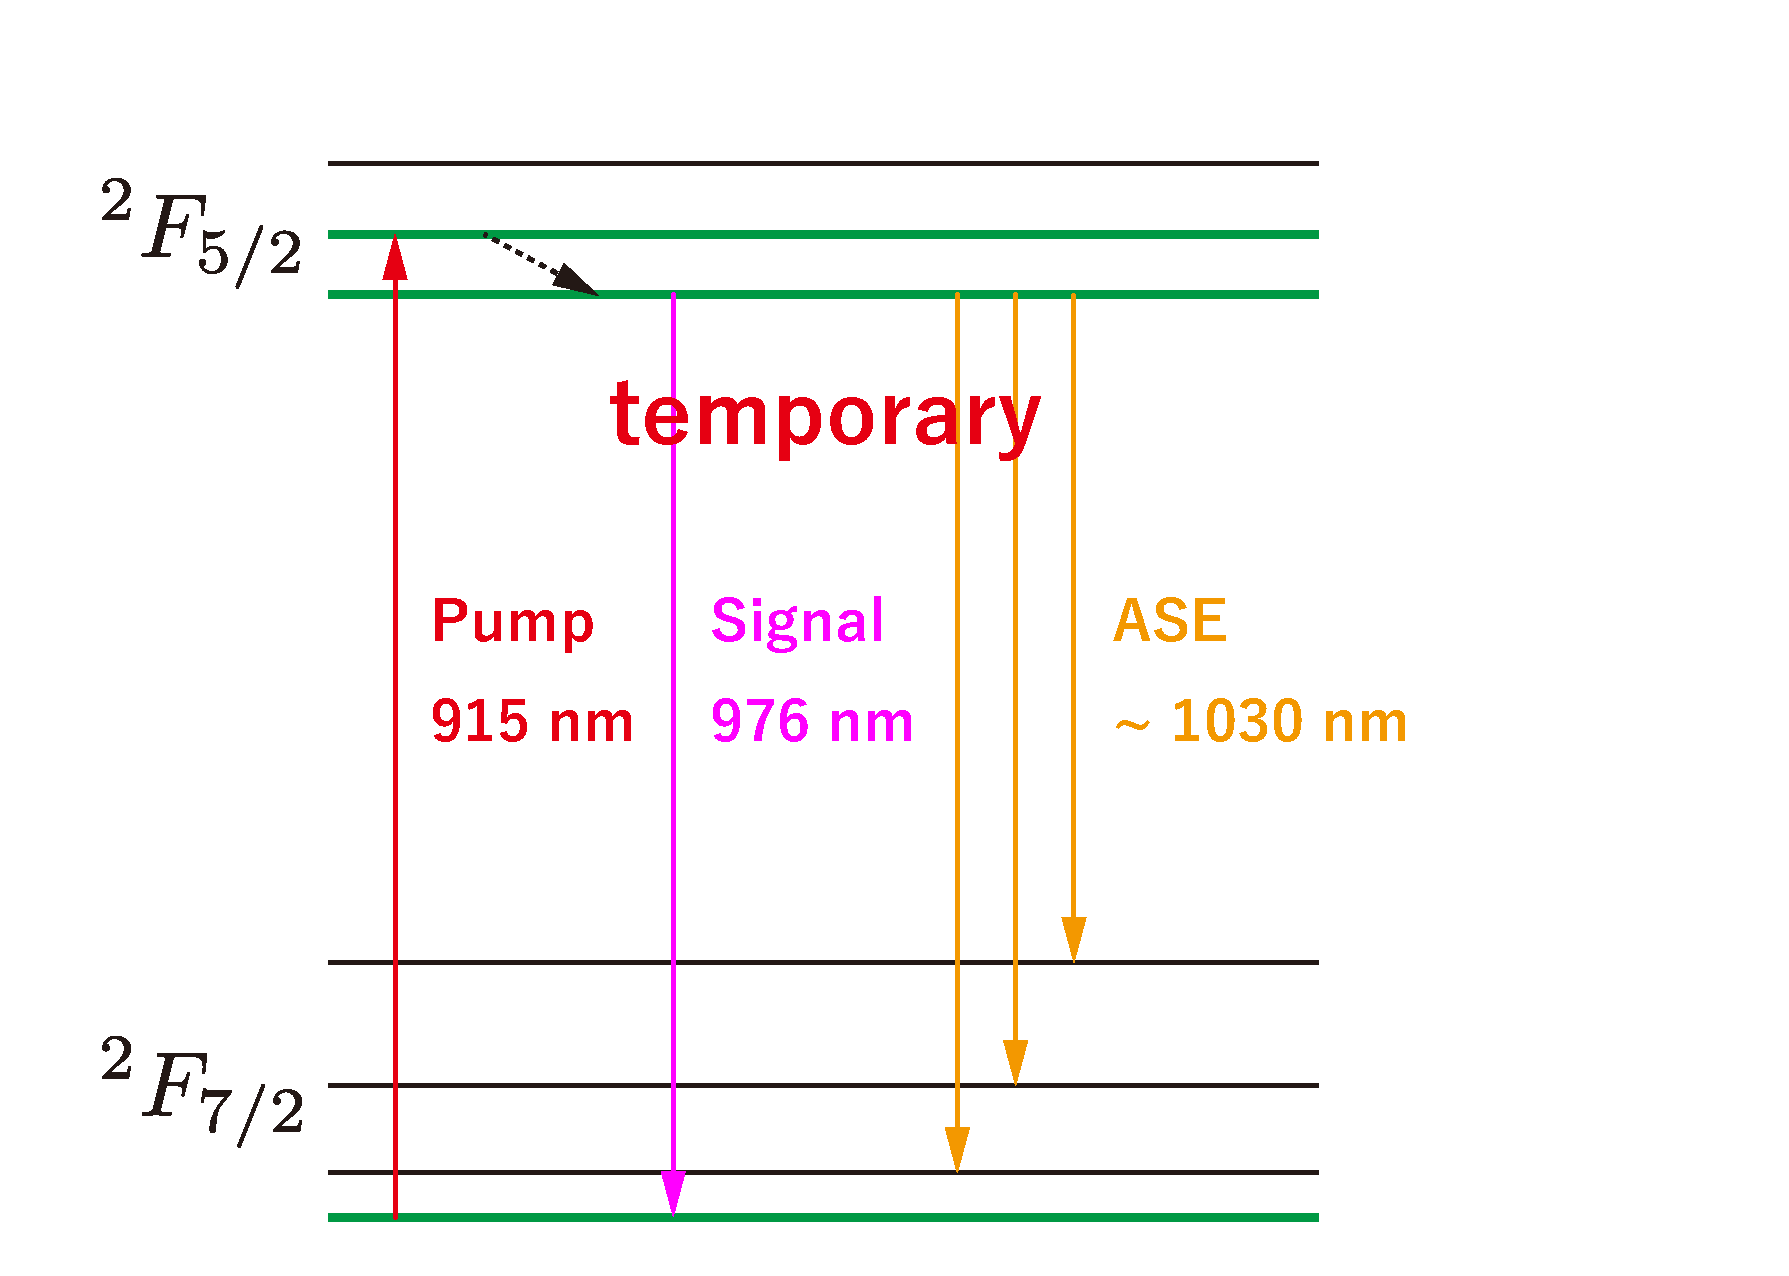
\includegraphics[keepaspectratio, width=0.9\linewidth]{./Figure/RelevantEnergyLevelOfYb3+InAluminosilicate}
    %\subcaption{}
  \end{minipage}
  \begin{minipage}[b]{0.5\linewidth}
    \centering
    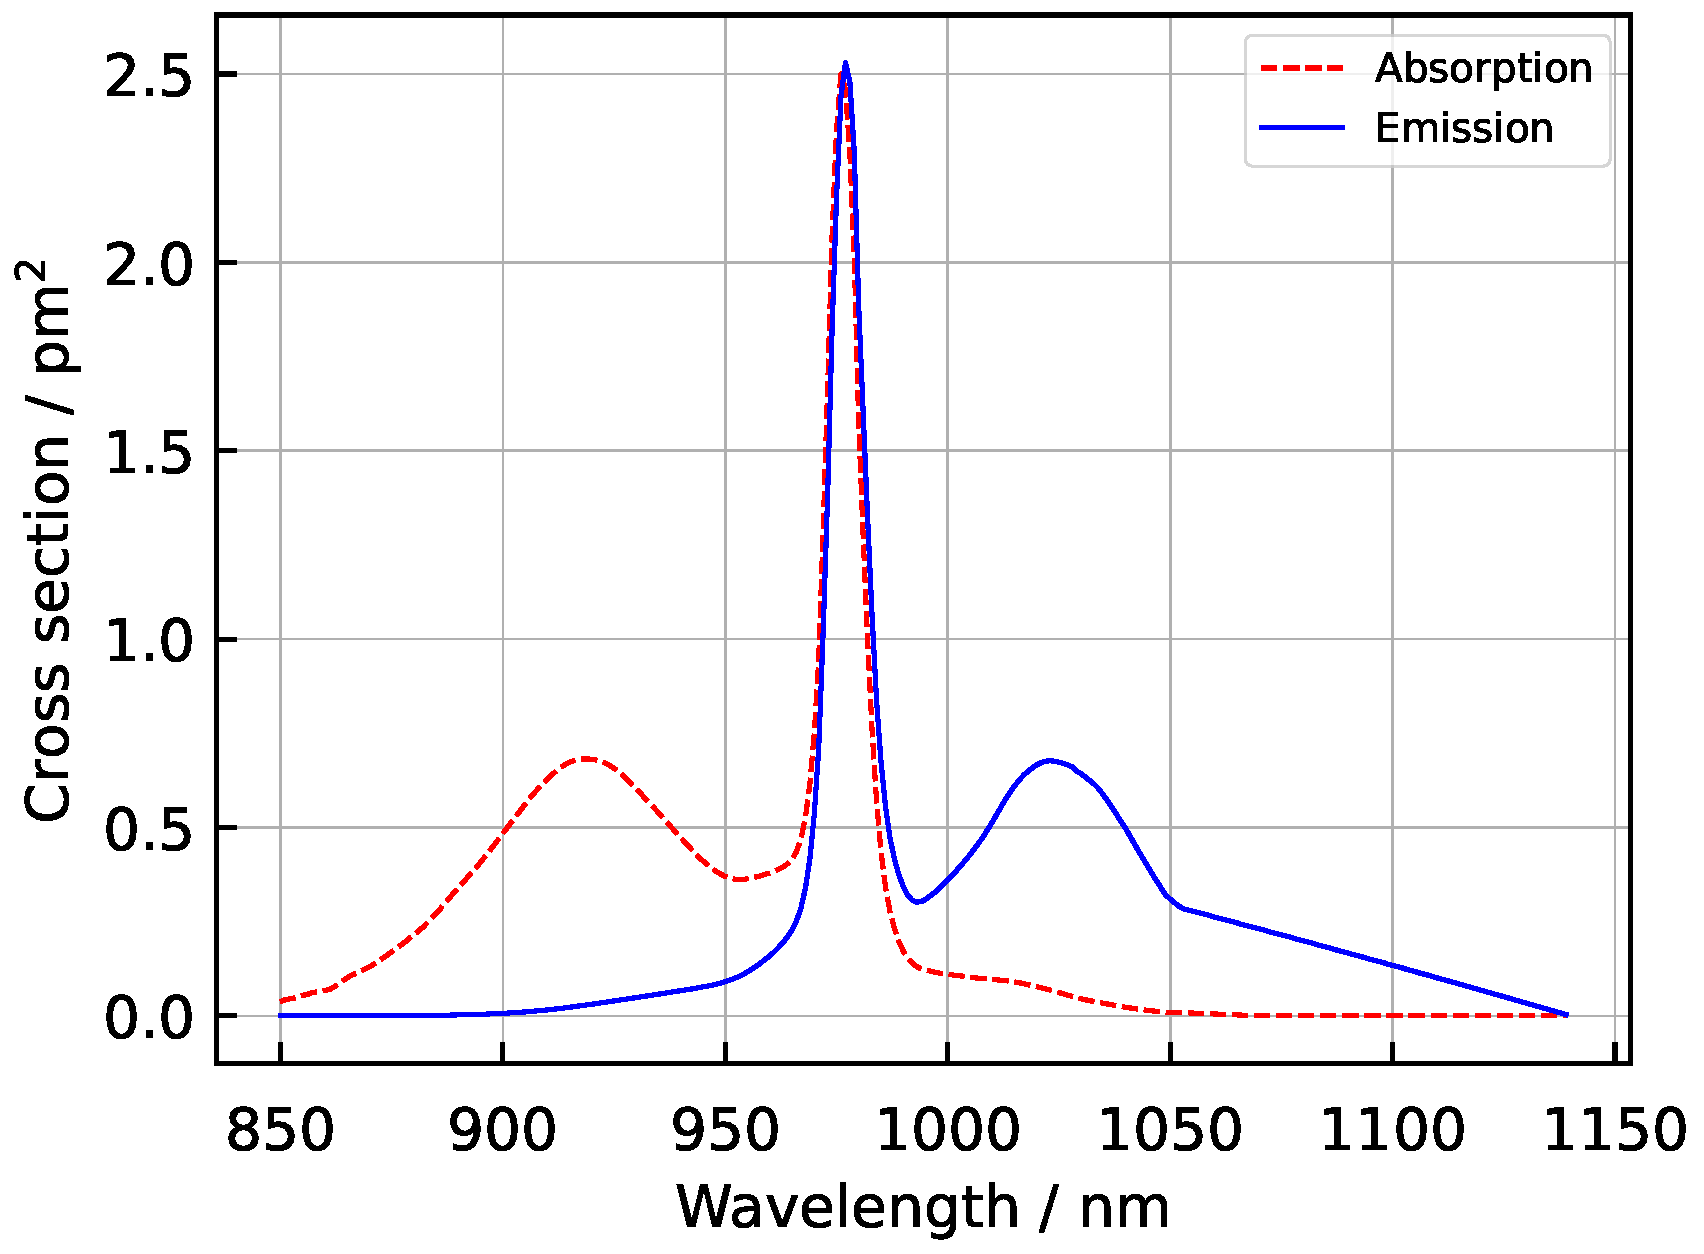
\includegraphics[keepaspectratio, width=0.9\linewidth]{./Figure/CrossSectionOfYb3+InAluminosilicate}
    %\subcaption{}
  \end{minipage}
  \caption{Relevant energy level and cross sections of Yb-doped fiber.}
  \label{fig:EnergylevelAndCrosssectionOfYb3+}
\end{figure}

For more detailed estimation for YDFA, numerical simulations are required.
We developed the simulation code based on the model in \cite{roeser200894}.
The simulations for forward and backward propagating pump, signal, and ASE were conducted according to the rate equation given by
\begin{equation}
  \begin{split}
    N &= N_{1} + N_{2}\\
    \dv{N_{2}}{t} &= \frac{1}{A_{core}} \frac{\lambda_{p}}{hc}\Gamma_{p} (P^{+}_{p} + P^{-}_{p}) (\sigma_{a}(\lambda_{p})N_{1} - \sigma_{e}(\lambda_{p})N_{2})\\
    &+ \frac{1}{A_{core}} \frac{\lambda_{s}}{hc}\Gamma_{s} (P^{+}_{s} + P^{-}_{s}) (\sigma_{a}(\lambda_{s})N_{1} - \sigma_{e}(\lambda_{s})N_{2})\\
    &+ \frac{1}{A_{core}} \frac{\lambda_{a}}{hc}\Gamma_{a} (P^{+}_{a} + P^{-}_{a}) (\sigma_{a}(\lambda_{a})N_{1} - \sigma_{e}(\lambda_{a})N_{2}) - \frac{N_{2}}{\tau},
  \end{split}
\end{equation} \todo{rewrite equations later}
and propagation equations in fiber are described as
\begin{align}
  \dv{P^{\pm}_{p}}{z} &= \pm\Gamma_{p}P^{\pm}_{p}(\sigma_{e}(\lambda_{p})N_{2} - \sigma_{a}(\lambda_{p})N_{1}) \mp \alpha P^{\pm}_{p}\\
  \dv{P^{\pm}_{s}}{z} &= \pm\Gamma_{s}P^{\pm}_{s}(\sigma_{e}(\lambda_{s})N_{2} - \sigma_{a}(\lambda_{s})N_{1}) \mp \alpha P^{\pm}_{s}\\
  \dv{P^{\pm}_{a}}{z} &= \pm\Gamma_{a}P^{\pm}_{a}(\sigma_{e}(\lambda_{a})N_{2} - \sigma_{a}(\lambda_{a})N_{1}) \mp \alpha P^{\pm}_{a} \pm 2\sigma_{e}(\lambda_{a})N_{2}\frac{hc^{2}}{\lambda_{a}^{3}}\Delta\lambda_{a}.
\end{align}
Here $N$ is the Yb-ion concentration, $N_{1}$ and $N_{2}$ are the population densities of the ground and excited state, respectively.
$\Gamma_{i} (i = p, s, a)$ is the overlapping factors for pump, signal, and ASE relative to the doped area, $A_{core}$ is the area of the doped area, $P^{\pm}_{i} (i = p, s, a)$ is the pump, signal, and ASE power, whose symbol $\pm$ corresponds to forward(+) and backward(-) propagation.
$\sigma_{e}, \sigma_{a}$ are the emission and absorption cross sections of Yb ions, and $\tau$ is the spontaneous lifetime of Yb ion in the excited state.
Comparison of simulation and experimental results will be discussed in a later Section \ref{sec:Discussion}.

\section{Experimental setup}
\subsection{976\,nm amplifier system}

\begin{figure}[h!]
  \centering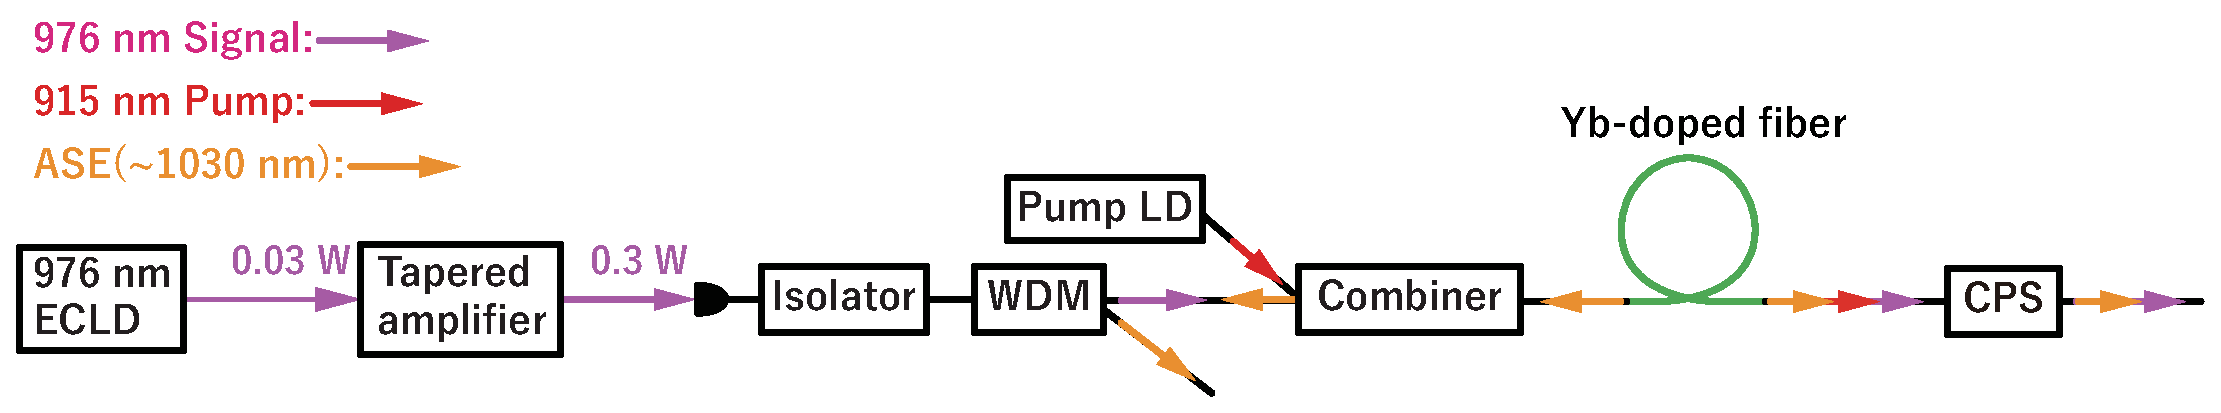
\includegraphics[width=\linewidth]{./Figure/976nmYDFASystem.eps}
  \caption{\SI{976}{\nm} YDFA system.}
  \label{fig:976YDFASystem}
\end{figure}

A schematic of the \SI{976}{\nm} YDFA system is shown in Fig.~\ref{fig:976YDFASystem}.
An external-cavity laser diode(ECLD) at \SI{976}{\nm} followed a tapered amplifier(TA) is used as a seed laser.
The output of seed laser is pre-amplified by the TA up to nearly \SI{1}{\W}, and coupled to the YDFA input which is a polarization maintaining(PM) fiber with a FPC/AC connector.
Owing to the spatial-mode mismatch of the output from TA, the power coupled to the input is only \SI{300}{\mW}.
The input of YDFA is fusion-spliced to an inline isolator and a wavelength division multiplexing(WDM) filter, which protect the seed laser from backward propagation light generated in a gain fiber.
The WDM which has three ports: a common port, a pass port, and a reflection port separates ASE around \SI{1020}{\nm} from signal path(common-pass) to the reflection port.
A fiber end of the reflection port is cleaved so that it is angled at least \ang{8} in order to prevent ASE from returning from the end to a gain fiber.
A \SI{915}{\nm} pump radiation is generated from fiber-coupled laser diode with output power of up to \SI{70}{\W}.
The pump laser is fixed on a water-cooled heatsink for stable operation.
A signal pump combiner, which has a signal port with PM fiber of \SI{6/125}{\um}, two pump ports with multimode fibers of \SI{105/125}{\um}, and a common port with double-cladding PM fiber of \SI{20/125}{\um}, combines the seed laser and the pump laser into the common port fiber.
The Yb-doped fiber fusion-spliced from the common port fiber of the combiner is rolled to approximately \SI{100}{\mm} in diameter and fixed on a water-cooled heatsink with a thermal conductive sheet.
For safe operation of the YDFA, all the bare glass cladding around the fusion-spliced points are recoated with low-refractive index polymer.
A residual pump power in the output of the Yb-doped fiber is removed by a cladding power stripper(CPS).
Amplified signal and ASE are collimated by pigtailed collimator, separated by a filter, and measured by power meters, respectively.


\subsection{1112\,nm amplifier system}

\begin{figure}[h!]
  \centering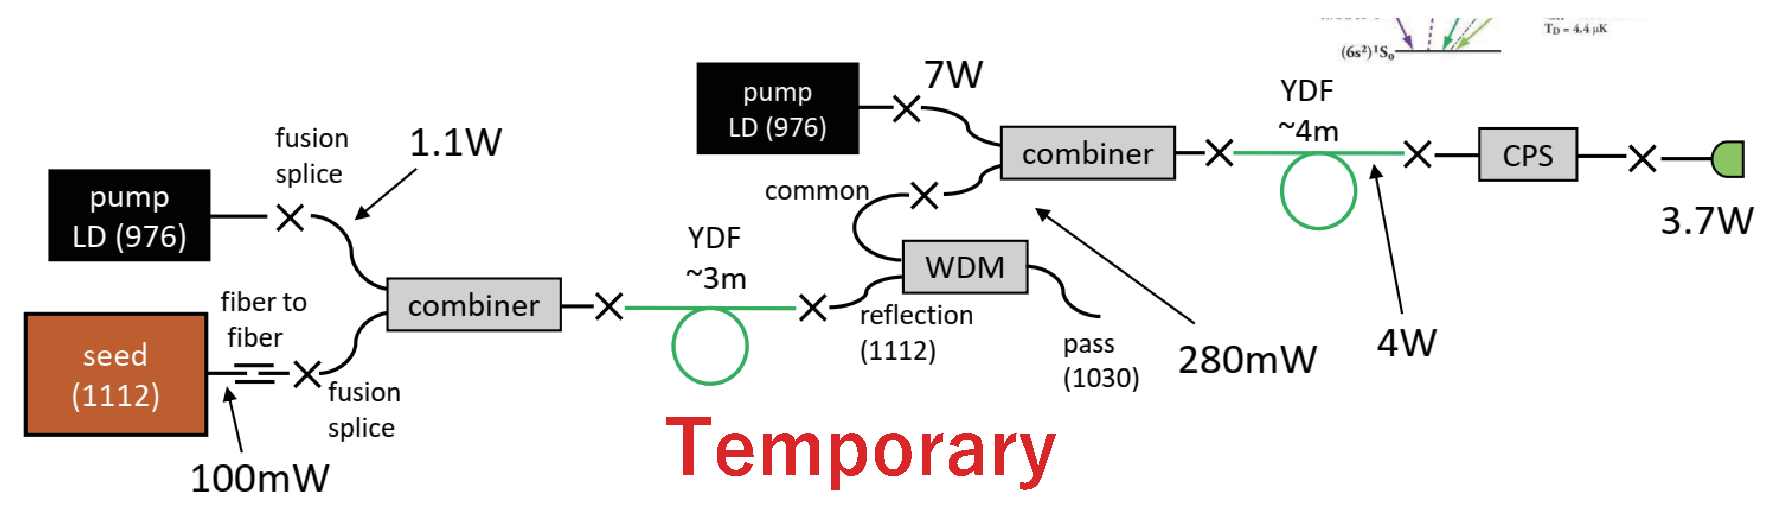
\includegraphics[width=\linewidth]{./Figure/1112nmYDFASystem_Temp.eps}
  \caption{\SI{1112}{\nm} YDFA system.}
  \label{fig:1112YDFASystem}
\end{figure}

A schematic of the \SI{1112}{\nm} YDFA system is shown in Fig.~\ref{fig:1112YDFASystem}.
The \SI{1112}{\nm} laser system is composed of a seed laser and two-stage YDFA.
A fiber laser at \SI{1112}{\nm}(Menlo systems Orange one-2) is used as the seed laser.
The output singlemode fiber with a FPC/AC connector is contacted to the input singlemode fiber of the first YDFA stage with a mating sleeve.
A coupled power into the input is about \SI{100?}{\mW}.
As pump lasers, two \SI{976}{\nm} fiber-coupled diode lasers based on an air-cooled heatsink with maximum outputs of \SI{7}{\W} are used.
The configuration of the first stage of \SI{1112}{\nm}YDFA is similar to the \SI{976}{\nm} system except for an isolator and fiber type.
The seed laser and the pump laser are combined into a double-cladding fiber of \SI{10/125}{\um} by a pump-signal combiner, and launched into the first Yb-doped fiber.
Before a second pump-signal combiner, the ASE around \SI{1020}{\nm} generated in first Yb-doped fiber is removed by a WDM.
The \SI{1112}{\nm} signal after WDM is \SI{300?}{\mW}.
The second Yb-doped fiber is rolled in a diameter of \SI{100?}{\mm}, and fixed inside an aluminum enclosure with thermal conductive sheet.
Temperature of the aluminum enclosure is controlled by peltier devices.
Similar to \SI{976}{\nm} system, the output of the second Yb-doped fiber is removed by CPS and collimated by pigtailed collimator.
The output power of the \SI{1112}{\nm} signal and the ASE near \SI{1020}{\nm} are obtained by measuring the output powers through long-pass filters with cut-on wavelengths at \SI{1100?}{\nm}.

\section{Experimental results}
\subsection{976\,nm YDFA}

\begin{figure}[h!]
  \begin{minipage}[b]{0.5\linewidth}
    \centering
    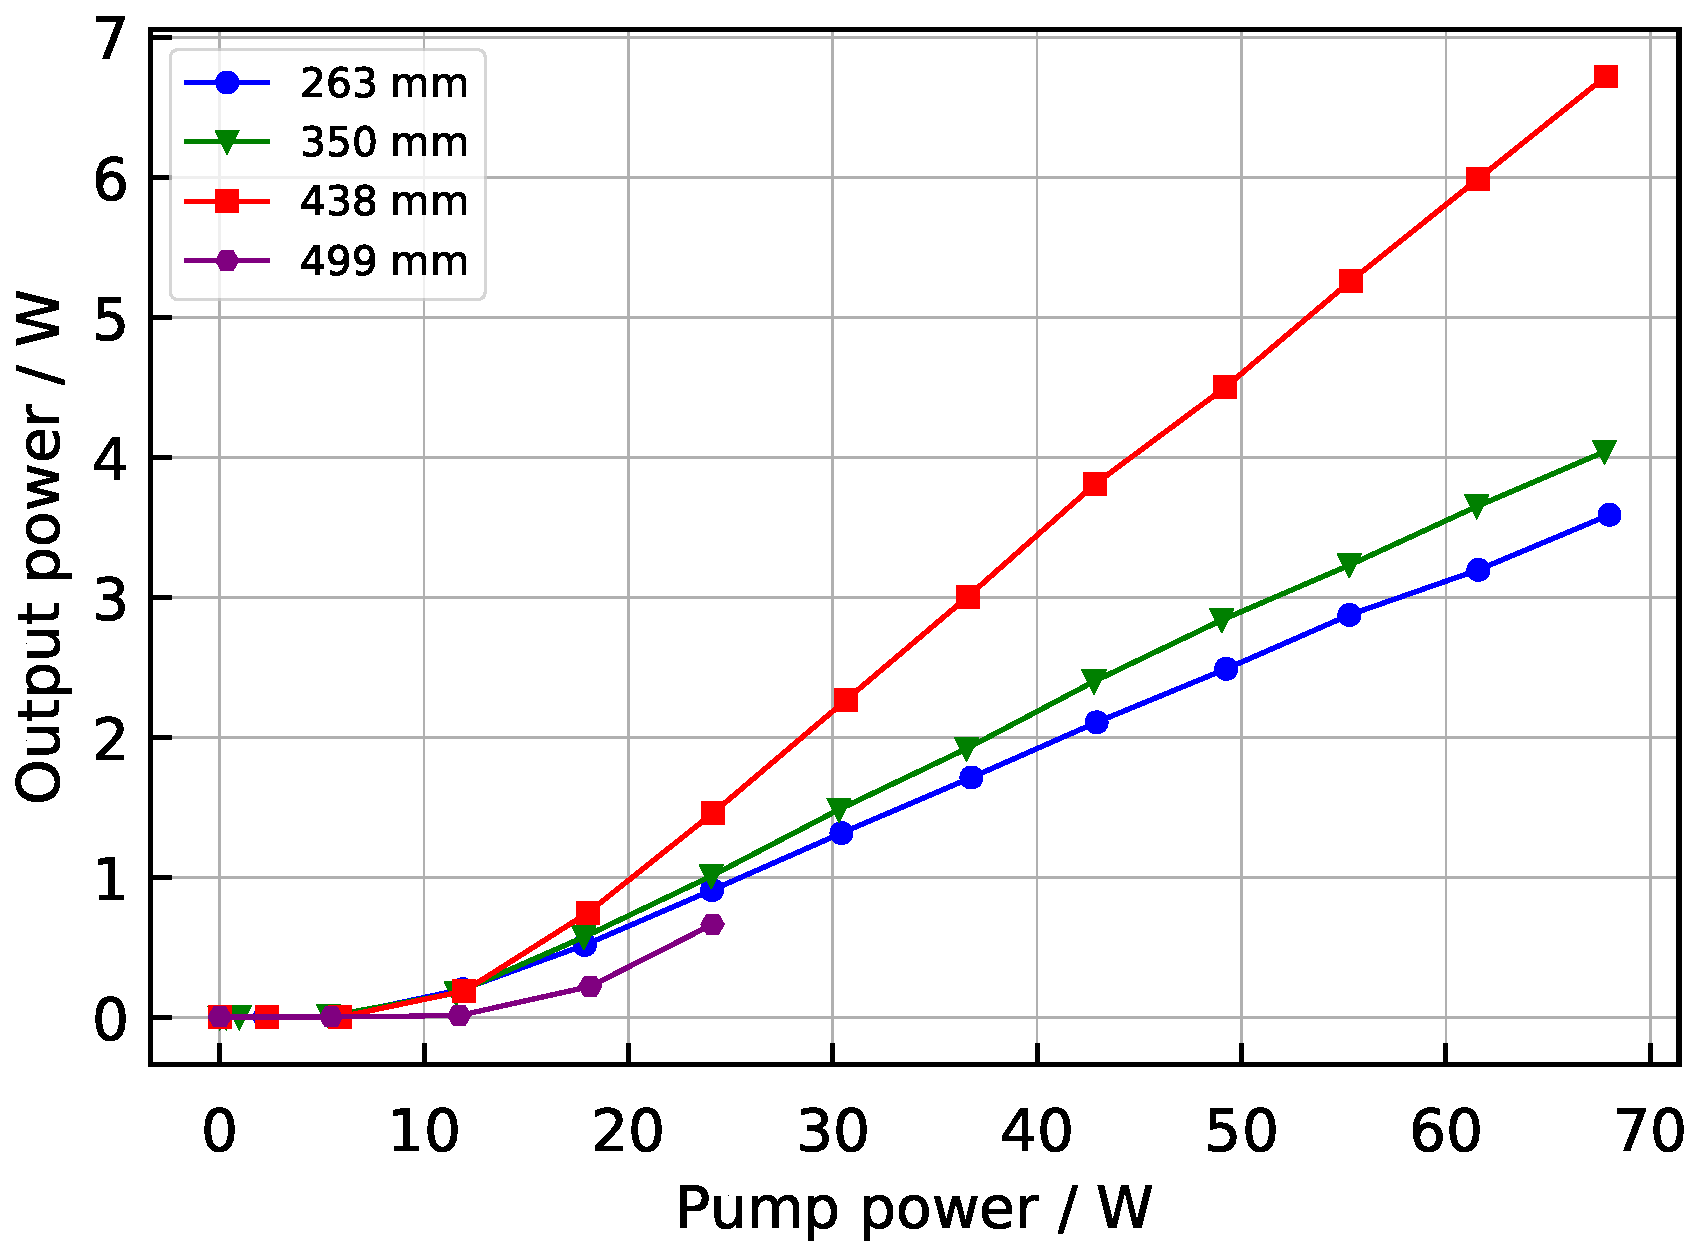
\includegraphics[keepaspectratio, width=0.9\linewidth]{./Figure/Yb1200-20-125DC-PM_SignalComparisonByLength_915Pump976Seed_Exp}
    \subcaption{}
  \end{minipage}
  \begin{minipage}[b]{0.5\linewidth}
    \centering
    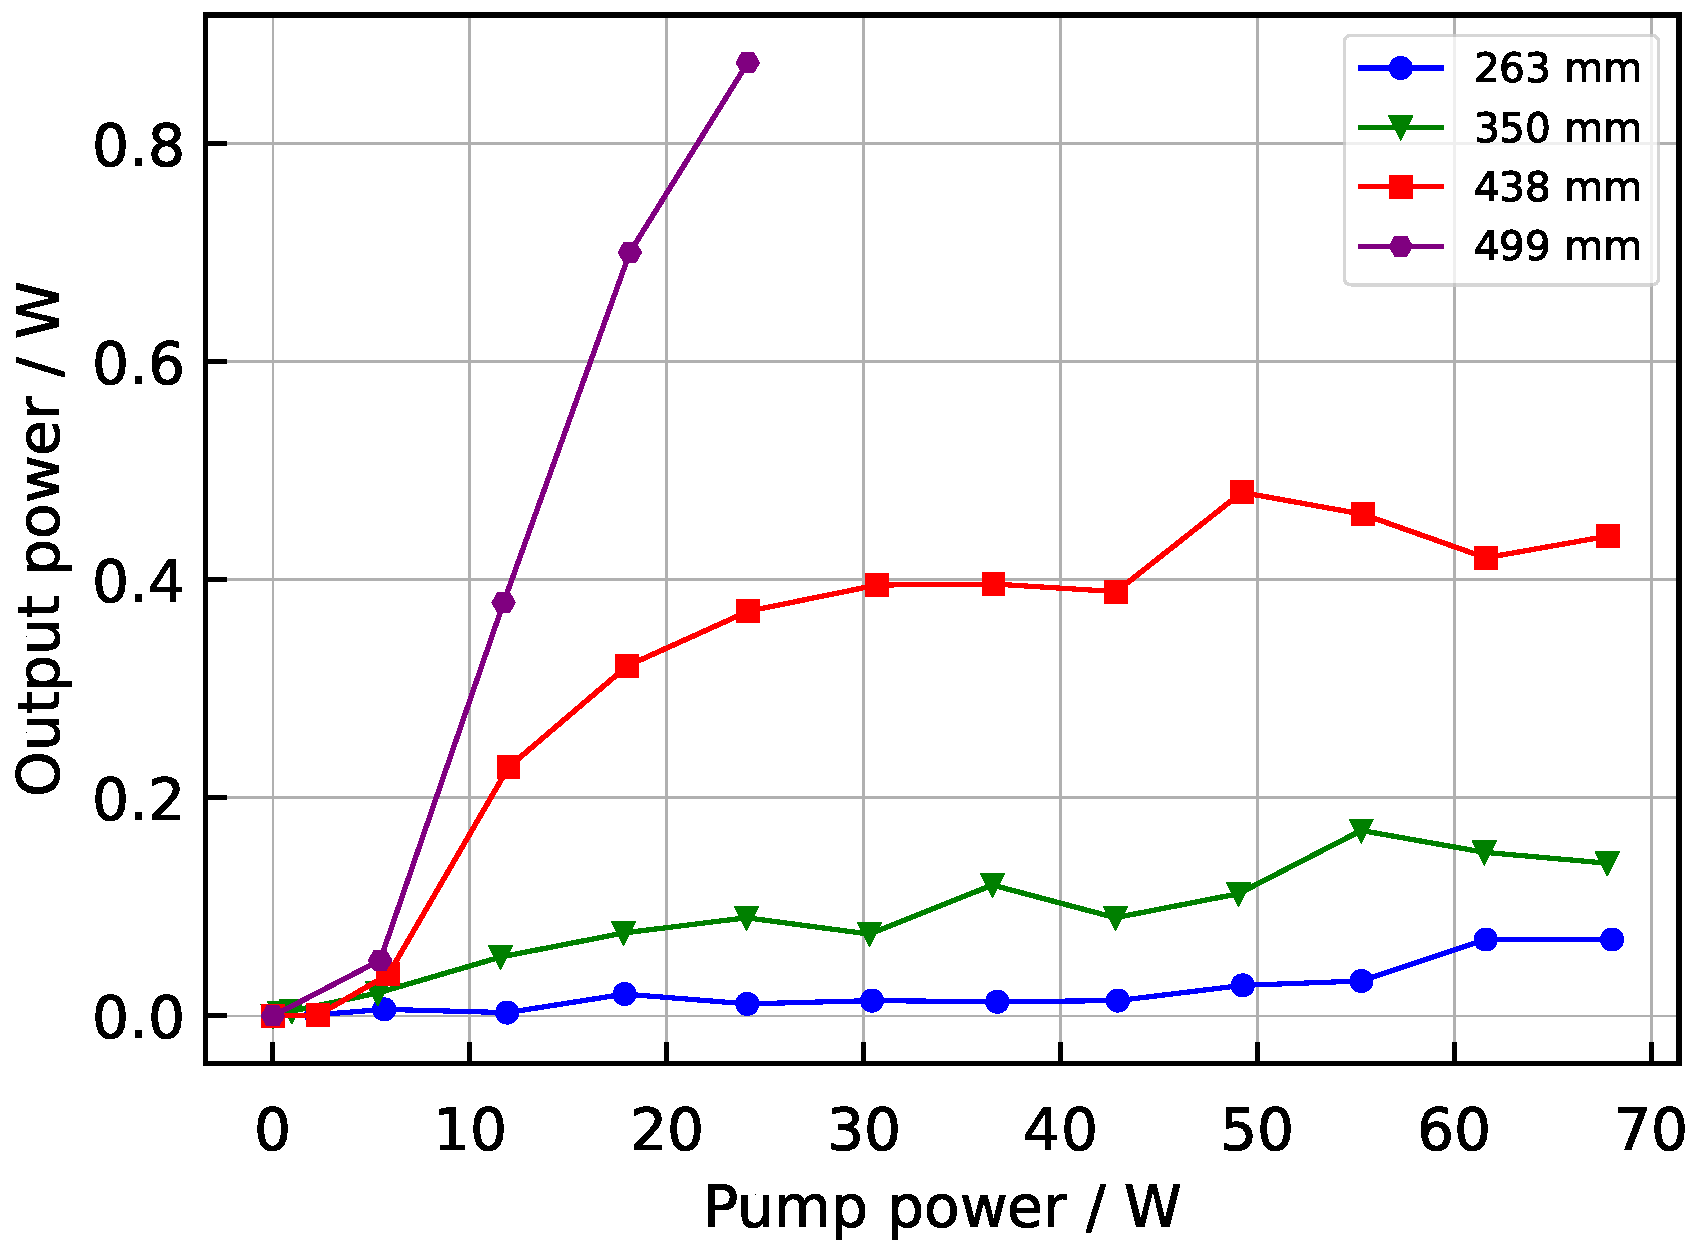
\includegraphics[keepaspectratio, width=0.9\linewidth]{./Figure/Yb1200-20-125DC-PM_ASEComparisonByLength_915Pump976Seed_Exp}
    \subcaption{}
  \end{minipage}
  \caption{Measured \SI{976}{\nm} and ASE around \SI{1020}{\nm} power as a function of the launched \SI{915}{\nm} pump power.}
  \label{fig:OutputComparisonOfNLIGHT976YDFA}
\end{figure}

The \SI{976}{\nm} and ASE near \SI{1020}{\nm} output power of the YDFA are shown in Fig.~\ref{fig:OutputComparisonOfNLIGHT976YDFA}.
In this measurement, we used a Yb-doped aluminosilicate fiber(nLIGHT, Yb1200-20/125DC-PM) as a gain fiber.
We tested \SI{263}{\mm}, \SI{350}{\mm}, \SI{438}{\mm}, and \SI{499}{\mm} long of the Yb-doped fibers at pump powers up to about \SI{70}{\W}.
As increasing the length of the Yb-doped fiber, the \SI{976}{\nm} output power increases, and reaches maximum at the \SI{438}{\mm} long fiber.
In the test of \SI{438}{\mm} long fiber, the \SI{976}{\nm} gain began to exceed 1 at the pump power of \SI{12}{\W}, and \SI{6.7}{\W} output of \SI{976}{\nm} was achieved with a slope efficiency of 0.12.
The maximum \SI{976}{\nm} gain corresponds to \SI{14.5}{\dB}.
The reason for the lower slope efficiency compared to YDFAs which has operating wavelength above \SI{1}{\um} is that the \SI{976}{nm} transition occurs between the lowest sublevel of the ground state and the lowest sublevel of the excited state in Yb ion.
In the test of \SI{499}{\mm} fiber, we applied the pump power less than \SI{25}{\W} because the ASE power significantly increased.

\begin{figure}[h!]
  \centering
  \begin{minipage}[b]{0.5\linewidth}
    \centering
    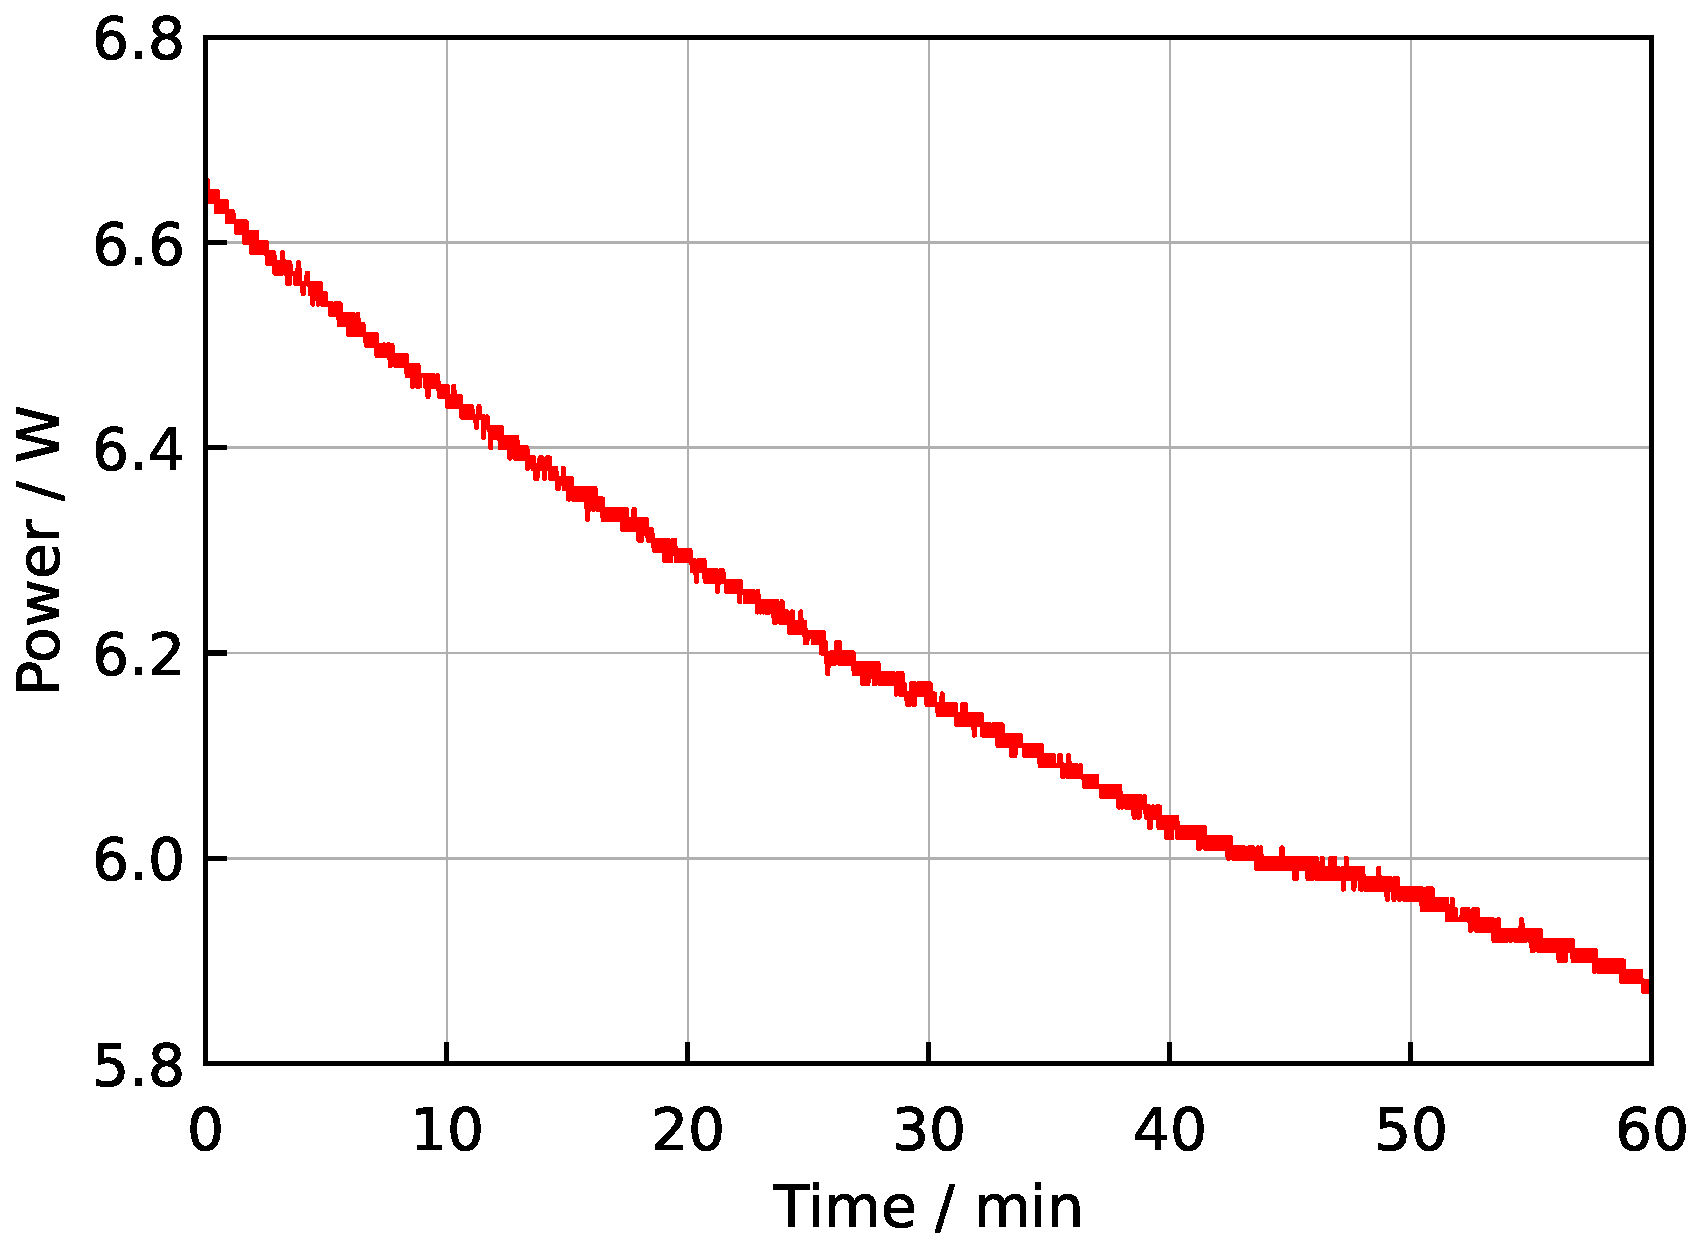
\includegraphics[keepaspectratio, width=0.9\linewidth]{./Figure/Yb1200-20-125DC-PM438mm_LongTermStability_915Pump70W976Seed0.24W_Exp}
    % \subcaption{}
  \end{minipage}
  \caption{The output power of the \SI{976}{\nm} YDFA with during \SI{60}{\minute}.}
  \label{fig:LongTermStabilityOfNLIGHT976YDFA}
\end{figure}
To measure the output stability of the \SI{976}{nm} YDFA, we logged the maximum output of the \SI{438}{mm} long fiber during \SI{60}{\minute}.
As the result shown in Fig.~\ref{fig:LongTermStabilityOfNLIGHT976YDFA}, the output of YDFA decayed in time to decrease by about 88\% of its original power after \SI{60}{\minute}.
This is mainly due to photodarkening caused by the high-inversion distribution of Yb ion \cite{paschotta1997Lifetime}.
Although the photodarkening is not fully understood, there are many proposals to mitigate the effect \cite{manek-honninger2007Photodarkening, zhao2019Elimination, engholm2008Preventing}.
To avoid power decay by photodarkening, we tested another Yb-doped fiber with phosphosilicate-glass core(Coractive, DCF-YB-20/128P-FAC).
\begin{figure}[h]
  \begin{minipage}[b]{0.5\linewidth}
    \centering
    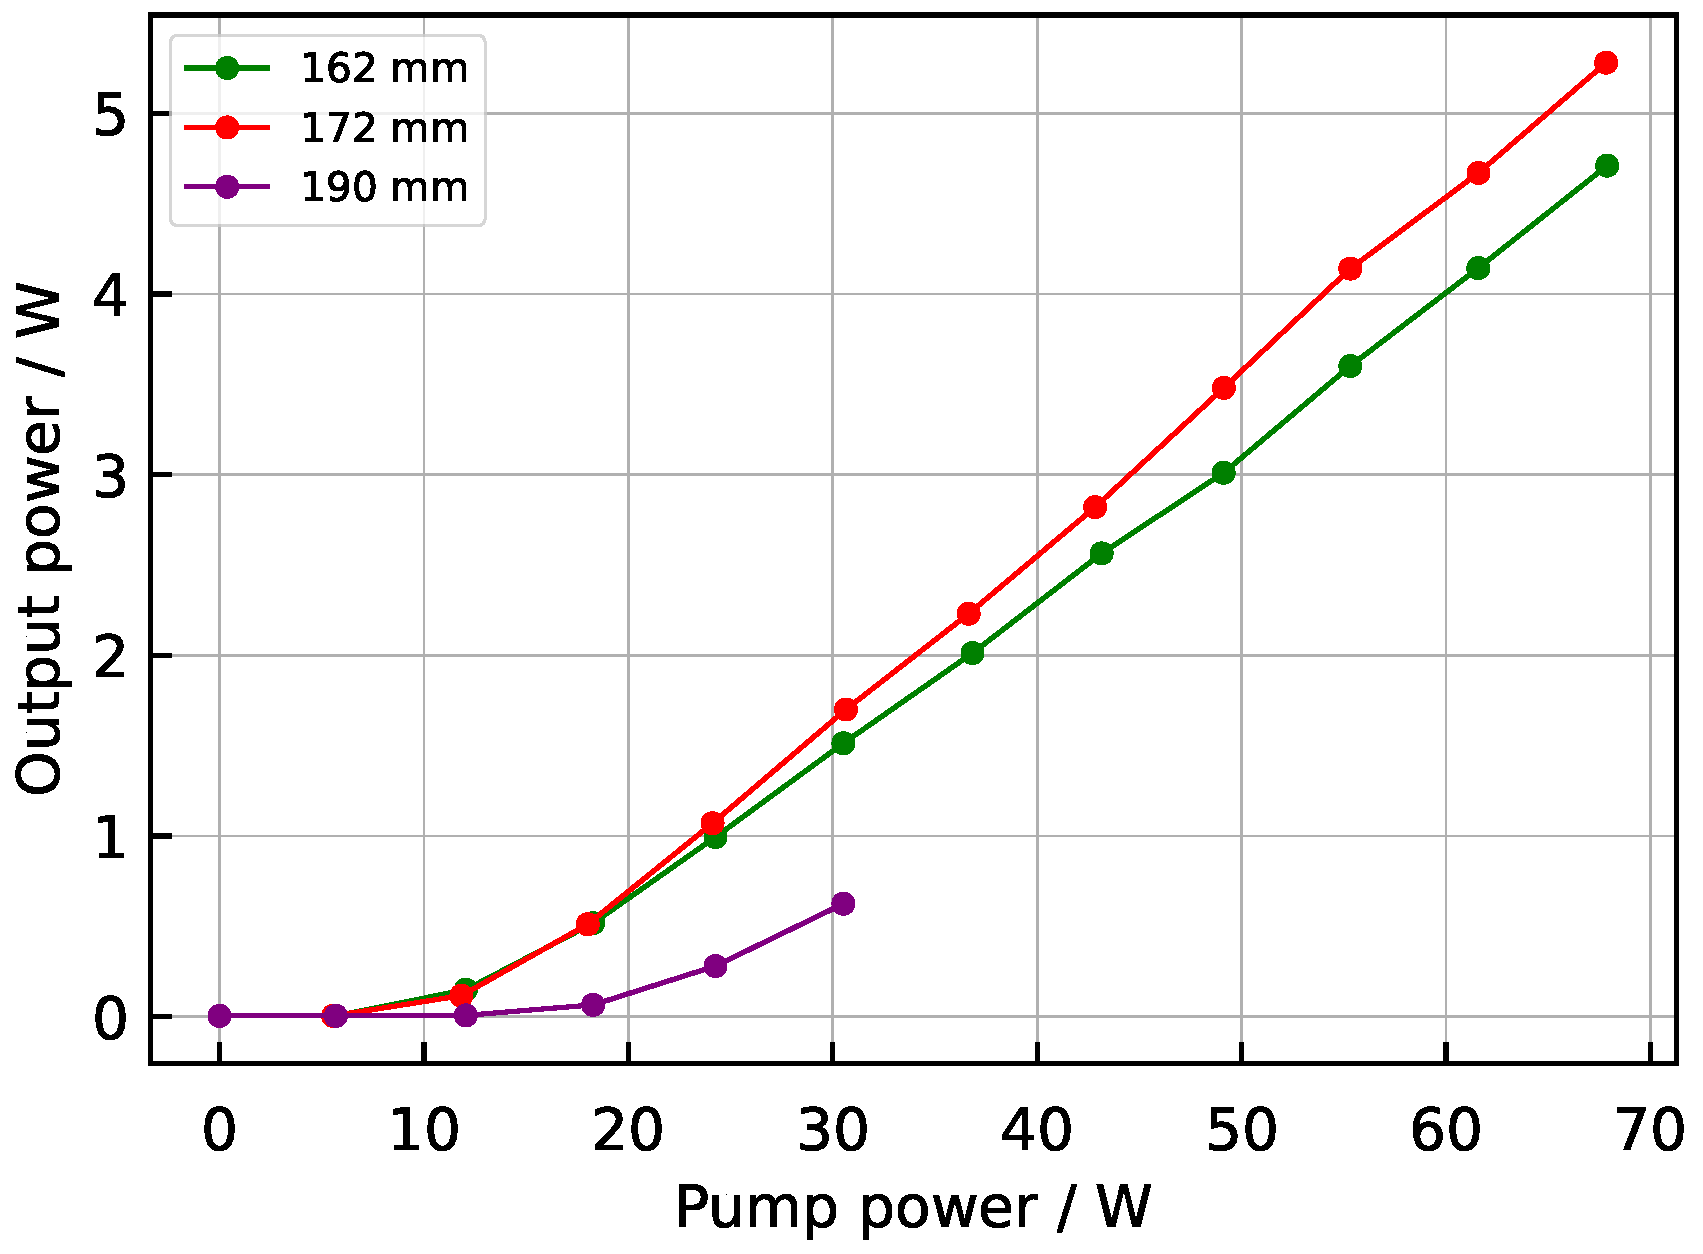
\includegraphics[keepaspectratio, width=0.9\linewidth]{./Figure/DCF-YB-20-128P-FAC172mm_SignalComparisonByLength_915Pump976Seed0.24W_Exp}
    \subcaption{}
  \end{minipage}
  \begin{minipage}[b]{0.5\linewidth}
    \centering
    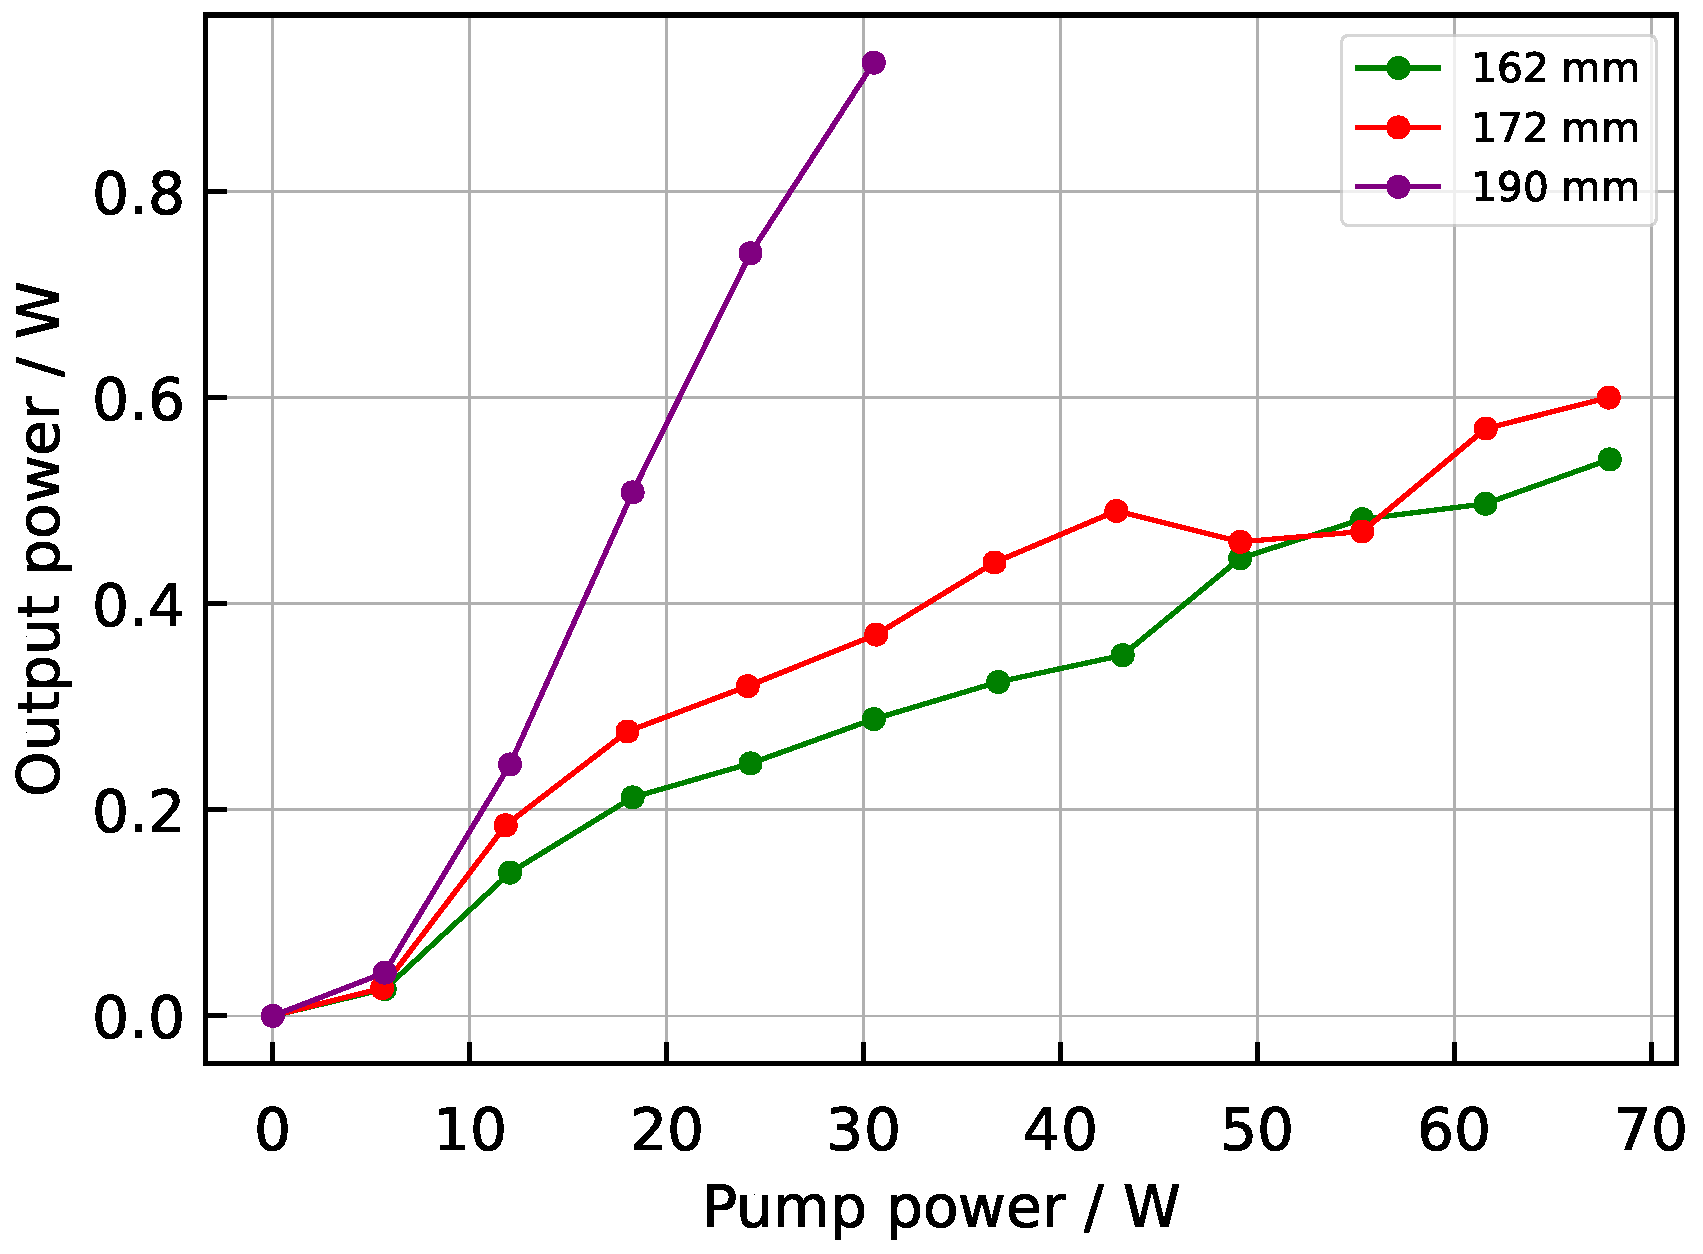
\includegraphics[keepaspectratio, width=0.9\linewidth]{./Figure/DCF-YB-20-128P-FAC172mm_ASEComparisonByLength_915Pump976Seed0.24W_Exp}
    \subcaption{}
  \end{minipage}
  \caption{Measured \SI{976}{\nm} and ASE around \SI{1020}{\nm} power as a function of the launched \SI{915}{\nm} pump power.}
  \label{fig:OutputComparisonOfCORACTIVE976YDFA}
\end{figure}
The output powers of YDFA with the \SI{162}{\mm}, \SI{172}{\mm}, and \SI{190}{\mm} long doped-phosphosilicate fiber are shown in the Fig.~\ref{fig:OutputComparisonOfCORACTIVE976YDFA}.
The \SI{976}{nm} output power reached a maximum of \SI{5.3}{\W} at the \SI{172}{\mm} length fiber.
Figure~\ref{fig:LongTermStabilityOfCORACTIVE976YDFA} shows \SI{976}{\nm} output stability of the \SI{172}{\mm} Yb-doped fiber.

\begin{figure}[h!]
  \centering
  \begin{minipage}[b]{0.5\linewidth}
    \centering
    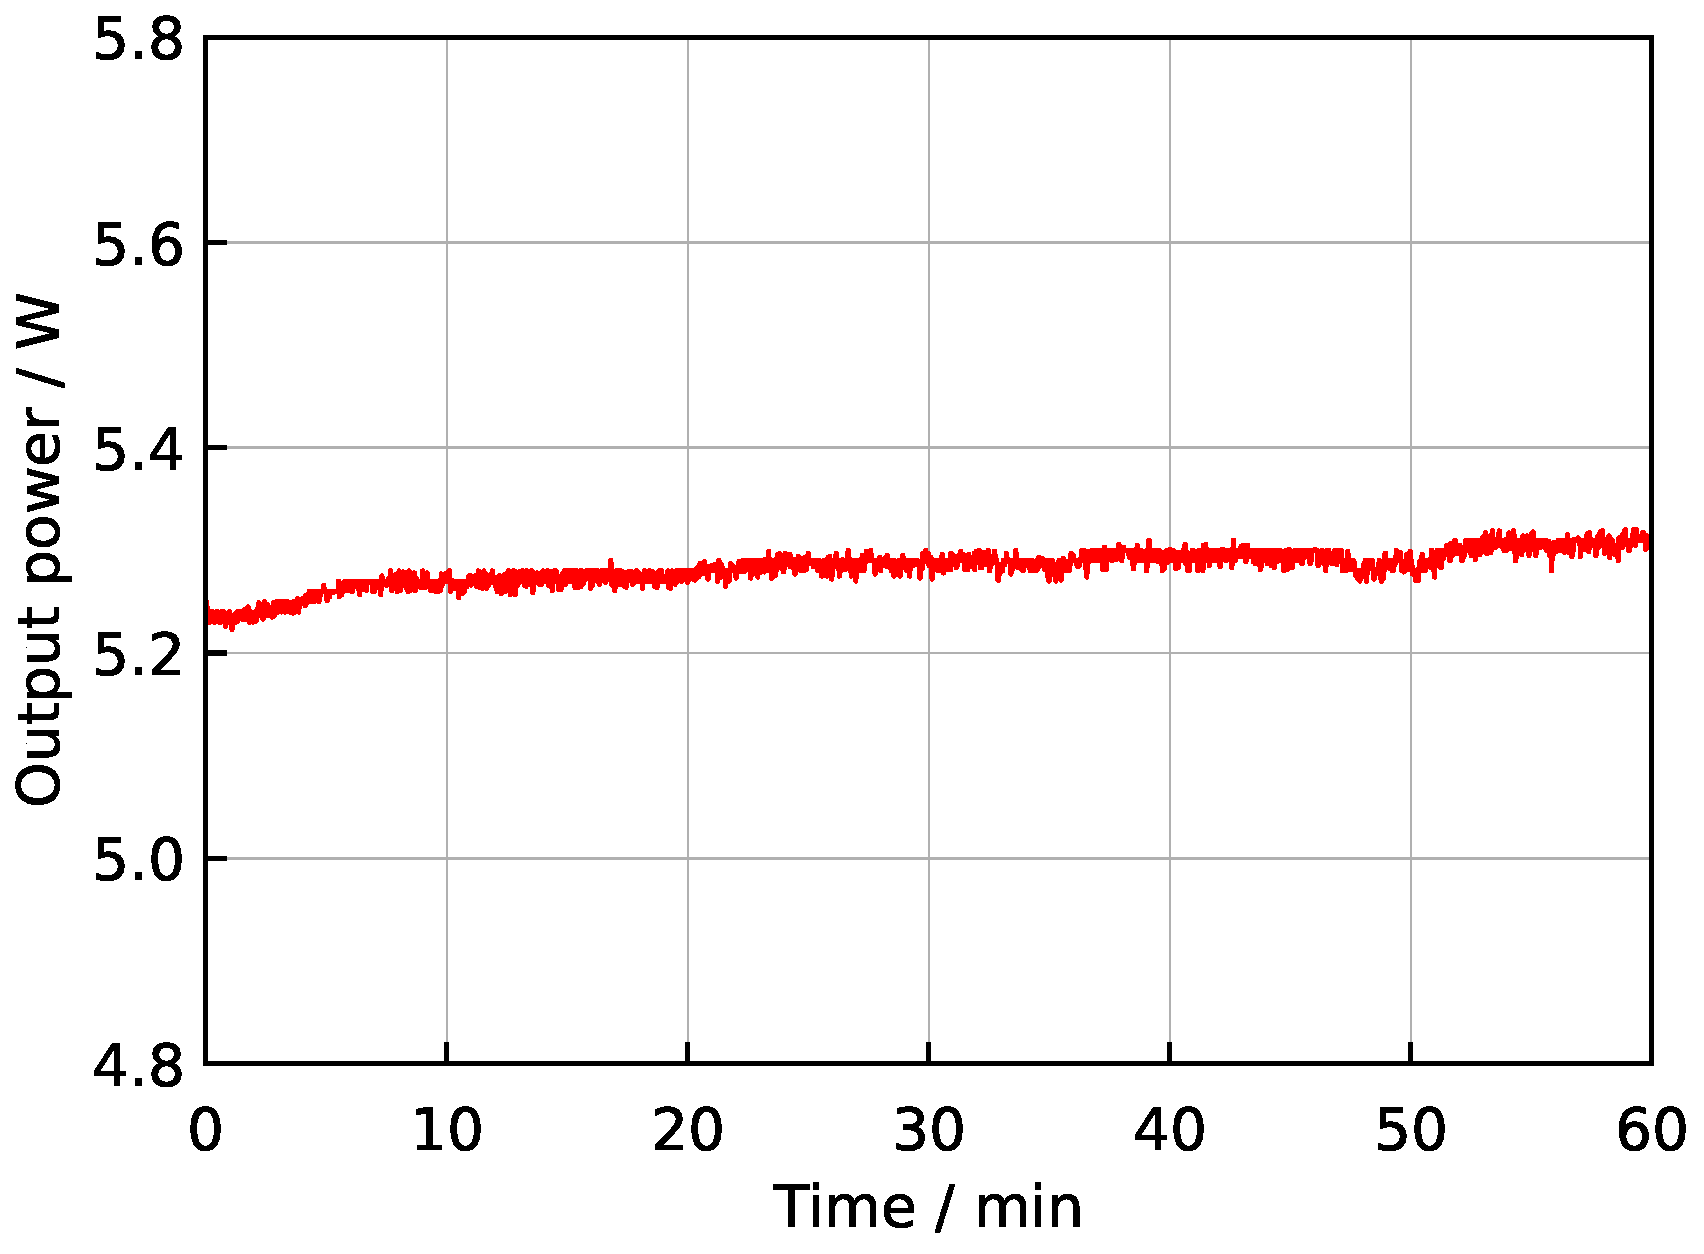
\includegraphics[keepaspectratio, width=0.9\linewidth]{./Figure/DCF-YB-20-128P-FAC172mm_SignalLongTermStability_915Pump70W976Seed0.24W_Exp}
    %\subcaption{}
  \end{minipage}
  \caption{The output power of the \SI{976}{\nm} YDFA during \SI{60}{\minute}.}
  \label{fig:LongTermStabilityOfCORACTIVE976YDFA}
\end{figure}


\subsection{1112\,nm YDFA}


\section{Comparison between numerical simulation and experimental results} \label{sec:Discussion}
\begin{figure}[h!]
  \centering
  \begin{minipage}[b]{0.5\linewidth}
    \centering
    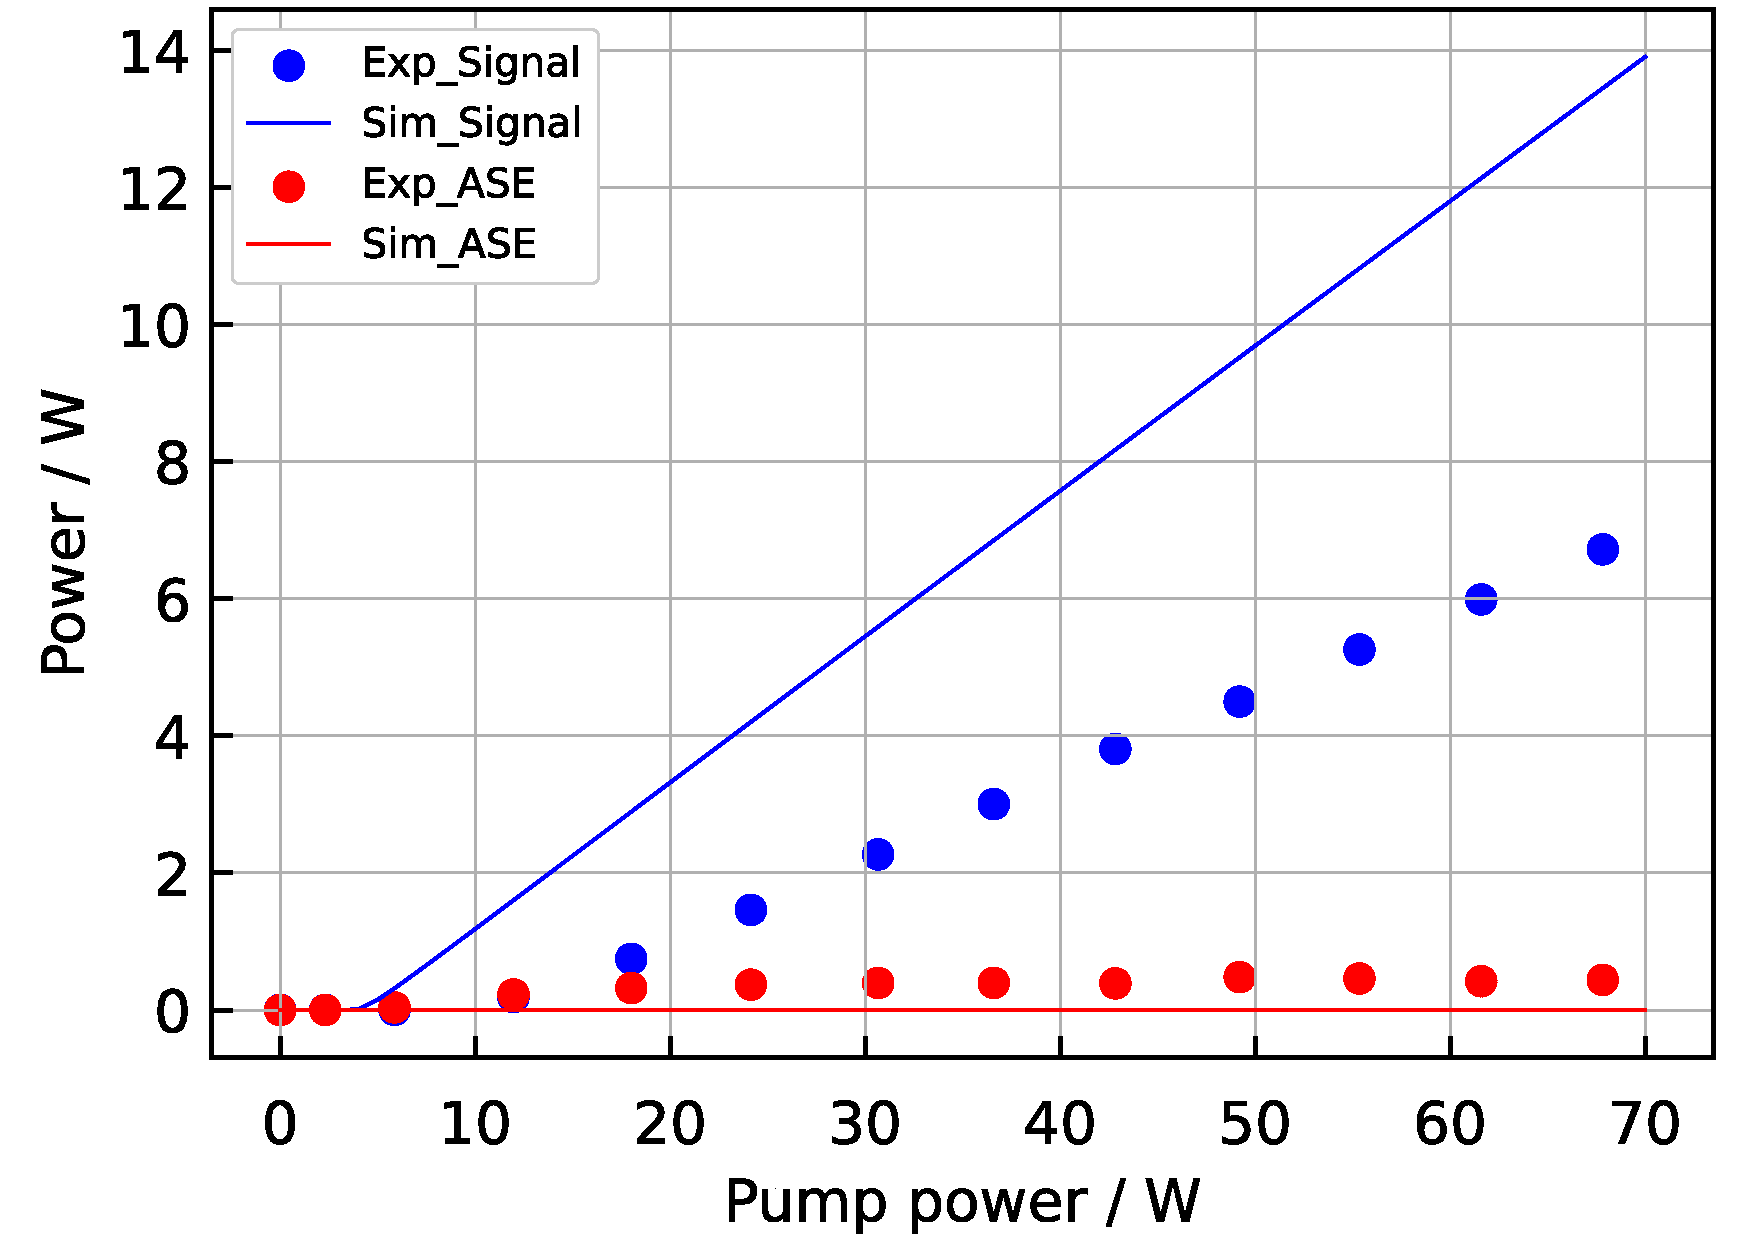
\includegraphics[keepaspectratio, width=0.9\linewidth]{./Figure/CompareSimAndExp_Yb1200-20-125DC-PM438mm_915Pump976Seed0.24W.pdf}
    %\subcaption{}
  \end{minipage}
  \caption{Comparison between numerical simulation and experimental results of the \SI{976}{\nm} YDFA.}
  \label{fig:ComparisonBetweenSimAndExpOf976YDFA}
\end{figure}

\section{Conclusion}
\begin{comment}
  The Universal Manuscript Template is based on the Express journal layout and will provide an accurate length estimate for \emph{Optics Express}, \emph{Biomedical Optics Express},  \emph{Optical Materials Express}, and our newest title \emph{OSA Continuum}
  \emph{Applied Optics}, JOSAA, JOSAB, \emph{Optics Letters}, \emph{Optica}, and \emph{Photonics Research} publish articles in a two-column layout
  To estimate the final page count in a two-column layout, multiply the manuscript page count (in increments of 1/4 page) by 60\%
  For example, 11.5 pages in the Universal Manuscript Template are roughly equivalent to 7 composed two-column pages
  Note that the estimate is only an approximation, as treatment of figure sizing, equation display, and other aspects can vary greatly across manuscripts
  Authors of Letters may use the legacy template for a more accurate length estimate.
\end{comment}

\begin{backmatter}

\bmsection{Funding}
JSPS KAKENHI Grant Number JP21K13944

\bmsection{Acknowledgments}


\end{backmatter}

%%%%%%%%%%%%%%%%%%%%%%% References %%%%%%%%%%%%%%%%%%%%%%%%%

%%%%%%%%%% If using BibTeX:
\bibliography{2022YDFA}

%%%%%%%%%% If preparing manually:
% \begin{thebibliography}{1}
% \newcommand{\enquote}[1]{``#1''}

% \bibitem{Zhang:14}
% Y.~Zhang, S.~Qiao, L.~Sun, Q.~W. Shi, W.~Huang, L.~Li, and Z.~Yang,
%   \enquote{Photoinduced active terahertz metamaterials with nanostructured
%   vanadium dioxide film deposited by sol-gel method,}
%   {\protect\JournalTitle{Optics Express}} \textbf{22}, 11070--11078 (2014).

% \bibitem{OSA}
% {Optical Society}, \enquote{{OSA Publishing},}
%   \url{http://www.osapublishing.org}.

% \bibitem{FORSTER2007}
% P.~Forster, V.~Ramaswamy, P.~Artaxo, T.~Bernsten, R.~Betts, D.~Fahey,
%   J.~Haywood, J.~Lean, D.~Lowe, G.~Myhre, J.~Nganga, R.~Prinn, G.~Raga,
%   M.~Schulz, and R.~V. Dorland, \enquote{Changes in atmospheric consituents and
%   in radiative forcing,} in \enquote{Climate Change 2007: The Physical Science
%   Basis. Contribution of Working Group 1 to the Fourth assesment report of
%   Intergovernmental Panel on Climate Change,}  S.~Solomon, D.~Qin, M.~Manning,
%   Z.~Chen, M.~Marquis, K.~B. Averyt, M.~Tignor, and H.~L. Miler, eds.
%   (Cambridge University Press, 2007).

% \end{thebibliography}

\end{document}
